\documentclass[12pt]{article}

\usepackage[a4paper,margin=2cm,top=2cm,bottom=2cm,xetex]{geometry}
\usepackage[utf8]{inputenc}
\usepackage{color,xcolor}
\usepackage{graphicx,algorithm,algorithmic,booktabs,multirow, multicol,float,amsfonts}
\usepackage{enumitem}
\usepackage{amssymb}
\usepackage{amsthm}
\usepackage{amsfonts}
\usepackage{mathtools}
\usepackage{flexisym}
\usepackage{algorithm}
\usepackage{algorithmic}
\usepackage{tabularx}
\usepackage{listings}
\usepackage{xepersian}
\usepackage{amsmath}
\usepackage{physics}

\DeclareFixedFont{\ttb}{T1}{txtt}{bx}{n}{12} % for bold
\DeclareFixedFont{\ttm}{T1}{txtt}{m}{n}{12}  % for normal

% Custom colors
\usepackage{color}
\definecolor{deepblue}{rgb}{0,0,0.5}
\definecolor{deepred}{rgb}{0.6,0,0}
\definecolor{deepgreen}{rgb}{0,0.5,0}

\usepackage{listings}

% Python style for highlighting
\newcommand\pythonstyle{\lstset{
language=Python,
basicstyle=\ttm,
morekeywords={self},              % Add keywords here
keywordstyle=\ttb\color{deepblue},
emph={MyClass,__init__},          % Custom highlighting
emphstyle=\ttb\color{deepred},    % Custom highlighting style
stringstyle=\color{deepgreen},
frame=none,                         % Any extra options here
showstringspaces=false
}}


% Python environment
\lstnewenvironment{python}[1][]
{
\pythonstyle
\lstset{#1}
}
{}

% Python for external files
\newcommand\pythonexternal[2][]{{
\pythonstyle
\lstinputlisting[#1]{#2}}}

% Python for inline
\newcommand\pythoninline[1]{{\pythonstyle\lstinline!#1!}}

%\usepackage{mathtools}

\DeclareFontFamily{U}{matha}{\hyphenchar\font45}
\DeclareFontShape{U}{matha}{m}{n}{ <-6> matha5 <6-7> matha6 <7-8>
matha7 <8-9> matha8 <9-10> matha9 <10-12> matha10 <12-> matha12 }{}
%\DeclareSymbolFont{matha}{U}{matha}{m}{n}
%
%\DeclareMathSymbol{\nvartrianglelefteq}{\mathrel}{matha}{"9E}
%\DeclareMathSymbol{\vartrianglelefteq}{\mathrel}{matha}{"9C}

\newcount\HWcnt
\def\ttmp#1#2#3#4#5#6#7#8#9|{\def\Wjob{#9}}%
\expandafter\ttmp\jobname |
\def\ttmp#1#2#3{\global\HWcnt=#2#3}
\expandafter\ttmp\Wjob

\settextfont[Scale = 1.0 ,
             BoldFont = *Bd ,
             ItalicFont = *It ,
             BoldItalicFont = *BdIt ,
             Extension = .ttf
            ]{XB Niloofar}
\ExplSyntaxOn
\cs_set_eq:NN
\etex_iffontchar:D
\tex_iffontchar:D
\cs_undefine:N \c_one
\int_const:Nn \c_one { 1 }
\ExplSyntaxOff
\setdigitfont[Scale = 1.0 ,
             BoldFont = *Bd ,
             ItalicFont = *It ,
             BoldItalicFont = *BdIt ,
             Extension = .ttf
            ]{XB Niloofar}
\renewcommand{\baselinestretch}{1.2}
\pagestyle{empty}

\makeatletter
\def\abj@num@i#1{%
	\ifcase #1\or الف\or ب\or ج\or د\or ه\or و\or ز\or ح\or ط\fi \ifnum #1=\z@ \abjad@zero \fi
}
\renewcommand{\theenumi}{\abjad{enumi}}
\renewcommand{\labelenumi}{\theenumi)}
\long\def\makeHead#1{%
	\begin{center}\large
		\begin{tabular}{@{}p{.33\linewidth}<{\hfill}@{}>{\hfil}p{.33\textwidth}<{}@{}>{\hfill}p{.33\textwidth}@{}}
            \textbf{تمرین ۳} & & \textbf{ایمان محمدی - 99102207} \\[.5ex]
            \textbf{نیم‌سال دوم ۱۴۰۱-۱۴۰۲} & &  \textbf{ زمان آپلود: #1}\\[.5ex] \hline\hline
		\end{tabular}
	\end{center}\smallskip
%	\def\theenumii{\arabic{enumii}}\def\theenumi{\alph{enumii}}\def\labelenumi{\theenumi)}\def\labelenumii{\theenumii)}%
}

\newcommand{\Rule}{\ \hfill\rule{\linewidth}{0.5pt}\hfill\ \par\vspace*{-2ex}\par}
\newcommand{\DescRule}{\ \hfill\rule{\linewidth}{1pt}\hfill\ \vspace*{-2ex}\par}
\def\rank{\mathop{\mathrm{rank}}\nolimits}

\begin{document}
\makeHead{۱۶ خرداد}
\begin{description}
%	\item{} \noindent
مهلت تحویل این تمرین ۰۸/۰۹/۱۴۰۱ است. شما در مجموع ترم  ۲۰ روز تاخیر مجاز دارید که مدیریت آن با خودتان است. در
ضمن برای هر تمرین شما تا سه روز بعد از ددلاین مجاز به ارسال پاسخ هستید و پس از آن به هیچ عنوان پاسخی از شما پذیرفته
نخواهد شد. پس از ساعات مجاز تاخیر، به ازای هر روز تاخیر،  ٣٠ درصد از نمره شما کسر خواهد شد.
	
%	\DescRule

	\item{\textbf{سوال 1.}} این بازی در واقع همان Minimax است و هر بازیکن سعی می‌کند در نوبت خودش، بدترین پاسخ را حذف کند و بهترین پاسخ را انتخاب کند. پس از آخر شروع می‌کنیم و به اول می‌رسیم.


در ابتدا راسی که یال k از پایین به آن وصل می‌شود را می‌خواهیم حذف کنیم و یک ۳ تایی به آن نسبت دهیم.

$$
(0.5 \times 300 + 0.5 \times 40 , 0.5 \times 40 + 0.5 \times 60 , 0.5 \times 0 + 0.5 \times 0)
$$

حالا تک‌تک حرکات حالت‌ها را تشخیص می‌دهیم.


بازیکن اول، حرکت k و پاداش ۲۰۰ را انتخاب می‌کند.


بازیکن سوم، حرکت I و پاداش ۱۵۰ را انتخاب می‌کند.


همچنین در یک جای دیگر، بازیکن سوم حرکت E را بین E و F انتخاب می‌کند.


همچنین بازیکن دوم بین حرکات G و H ، حرکت G را انتخاب می‌کند.


حالا در ادامه و در راسی که C به آن وصل می‌شود از پایین، باید احتمال‌ها را به عدد صحیح تبدیل کنیم و امید ریاضی پاداش‌های این راس بدست می‌آید:

$$
\frac{1}{3} \times 50 + \frac{2}{3} \times 200 , \frac{1}{3} \times 20 + \frac{2}{3} \times 50 , \frac{1}{3} \times 150 + \frac{2}{3} \times 0
$$

$$
= (150, 40, 50)
$$

در نتیجه بازیکن دوم بین حرکات C و D ، حرکت D را انتخاب می‌کند.


در ادامه و در راسی که B به آن وصل می‌شود از پایین، باید احتمال‌ها را به عدد صحیح تبدیل کنیم و امید ریاضی پاداش‌های این راس بدست می‌آید:

$$
0 + \frac{1}{10} \times 1000 , 0 + \frac{1}{10} \times 1500 , 0 + \frac{1}{10} \times 500
$$

$$
= (100, 150, 50)
$$

در نتیجه بازیکن اول بین حرکات A و B ، حرکت A را انتخاب می‌کند.

پس تعادل نش این بازی به کمک استقرای بازگشتی می‌شود:

$$
1A2D3E
$$

در واقع نیز استراتژی هر بازیکن بدین شکل است که بازیکن اول، A و K را انتخاب می‌کند، بازیکن دوم، D و G را انتخاب می‌کند و بازیکن سوم نیز I و E را انتخاب می‌کند.




	
	\Rule
	
	\item{\textbf{سوال 2.}} اثبات می‌کنیم در هر بازی متقارن، اگر
$
a_{i, i} > a_{i, j}
$
به ازای تمامی
$
i \neq j
$
برقرار باشد، آنگاه استراتژی خالص i یک استراتژی پایدار تکاملی است.

در حالت کلی، برای اثبات اینکه یک استراتژی خالص در یک بازی یک استراتژی پایدار تکاملی

\lr{(Evolutionary Stable Strategy - ESS)}
است، باید دو شرط را بررسی کنیم:


۱. استراتژی خالص
\lr{i}
باید برنده استراتژی خالص
\lr{j}
را وقتی بقیه بازیکنان استراتژی
\lr{i}
را انتخاب کرده باشند، برابر یا بیشتر از استراتژی
\lr{j}
کند.

۲. اگر استراتژی
\lr{i}
و
\lr{j}
هر دو به یک اندازه برنده باشند، آنگاه استراتژی
\lr{i}
باید برنده استراتژی
\lr{j}
را وقتی بقیه بازیکنان استراتژی
\lr{j}
را انتخاب کرده باشند، بیشتر از استراتژی
\lr{j}
کند.

بنابراین، برای اثبات این موضوع برای یک بازی متقارن، کافیست دو شرط فوق را برای ماتریس بازی بررسی کنیم. اگر ماتریس بازی به گونه ای باشد که 
$a_{i, i} > a_{i, j}$
برای همه 
$i ≠ j$
، بنابراین این دو شرط برقرار هستند و استراتژی
\lr{i}
یک استراتژی پایدار تکاملی
\lr{(ESS)}
است.

همچنین این موضوع به طور کلی نشان می دهد که در یک بازی متقارن، استراتژی 
\lr{i}
که بیشترین پی‌آف
\lr{(payoff)}
را به بازیکن می‌دهد (یعنی 
$a_{i, i}$
بیشترین مقدار را دارد) یک استراتژی پایدار تکاملی است.


برای مثال در این بازی:
\begin{center}	
	\begin{array}{c|cc}
		& 1 & 2 \\ \hline
		1 & a_{1, 1} & a_{1, 2} \\
		2 & a_{2, 1} & a_{2, 2} \\
	\end{array}
\end{center}	

این ماتریس بازی است که دو استراتژی خالص دارد: استراتژی 1 و استراتژی 2 . 
در یک بازی متقارن،
$a_{i, j} = a_{j, i}$
برقرار است. اگر شرایط مساله برقرار باشد که 
$a_{1, 1} > a_{1, 2}$ و $a_{2, 2} > a_{2, 1}$
، بنابراین هر دو استراتژی پایدار تکاملی
\lr{(ESS)}
هستند.

برای مثال، فرض کنید
$a_{1, 1} = 3$، $a_{1, 2} = 2$، $a_{2, 1} = 2$ و $a_{2, 2} = 3$
. 
در این حالت، هر دو استراتژی
\lr{(ESS)}
هستند. چرا که اگر همه بازیکنان استراتژی 1 را انتخاب کنند، هر بازیکنی که به استراتژی 2 تغییر کند، پاداش کمتری دریافت می‌کند و برعکس.


	
	\Rule
	
	\item{\textbf{سوال 3.}} سوال ۳

برای پیدا کردن تعادل نش در بازی دو نفره، ما ابتدا باید بازی را به صورت یک جدول سودمندی نمایش دهیم. در این بازی، مجموعه اعمال ممکن برای هر بازیکن عدد انتخابی از مجموعه 1 تا k است. بنابراین، جدول سودمندی بازی به صورت یک جدول
$k \times k$
خواهد بود.

سودمندی هر بازیکن را می‌توان با توجه به این که آیا اعداد انتخابی توسط آن‌ها با هم برابر است یا خیر تعیین کرد. اگر حمید و مجید عدد یکسانی را انتخاب کنند، مجید به حمید 1 ریال می‌دهد. در این صورت سودمندی حمید 1 خواهد بود و سودمندی مجید 
$-1$
خواهد بود. در غیر این صورت، سودمندی هر دو بازیکن 0 خواهد بود.

یک استراتژی ترکیبی برای یک بازیکن استراتژی‌ای است که بازیکن در آن به جای انتخاب یک عمل خاص، احتمالاتی را برای انتخاب هر عمل مشخص می‌کند. بنابراین، برای این بازی، یک استراتژی ترکیبی به این معنی است که حمید و مجید احتمالاتی را برای انتخاب هر عدد از 1 تا k مشخص می‌کنند.

اگر استراتژی ترکیبی حمید و مجید به ترتیب p و q باشد، سودمندی حمید
$E_p(q)$
و سودمندی مجید
$E_q(p)$
خواهد بود. این بازی یک تعادل نش دارد اگر و فقط اگر هیچ یک از بازیکنان نتوانند سودمندی خود را با تغییر استراتژی خود افزایش دهند. به عبارت دیگر، اگر 
$p*$
و
$q*$
تعادل نش باشد، آنگاه برای هر استراتژی p و q داریم:

$E_p(q*) \leq E_p*(q*)$ 
و
$E_q(p*) \leq E_q*(p*)$

در این بازی، تعادل نش وجود دارد اگر و فقط اگر
$p*$
و
$q*$
به گونه‌ای باشند که حمید و مجید به صورت تصادفی عددی از 1 تا k انتخاب می‌کنند. به عبارت دیگر، اگر
$p* = (\frac{1}{k}, \frac{1}{k}, ..., \frac{1}{k})$
و
$q* = (\frac{1}{k}, \frac{1}{k}, ..., \frac{1}{k})$
باشد. در این صورت، سودمندی انتظاری هر دو بازیکن برابر با 0 خواهد بود و هیچ یک از آن‌ها نمی‌توانند سودمندی خود را با تغییر استراتژی خود افزایش دهند.

می‌توان نشان داد که این تعادل تنها تعادل نش بازی است. اگر یک استراتژی تعادل نش دیگر وجود داشته باشد، باید بتوان سودمندی انتظاری حمید یا مجید را افزایش داد. اما، اگر حمید یا مجید احتمال بیشتری را برای انتخاب یک عدد خاص قرار دهند، بازیکن دیگر می‌تواند با انتخاب همان عدد سودمندی خود را افزایش دهد. بنابراین، تنها تعادل نش که در این بازی وجود دارد تعادلی است که در آن هر دو بازیکن به صورت تصادفی عددی از 1 تا k انتخاب می‌کنند.

	
	\Rule
	
	\item{\textbf{سوال 4.}} \subsection*{الف}

در این درخت، راس اول نمایانگر انتخاب اولیه عدد 
$\alpha$
است که می‌تواند یا ۱ یا -۱ باشد. 


سپس بازیکن اول (بازیکن 
$x$
) می‌تواند از میان ۱، ۲ یا ۴ انتخاب کند. 


بعد از انتخاب بازیکن اول، بازیکن دوم (بازیکن
$y$
) همچنین می‌تواند از میان ۱، ۲ یا ۴ انتخاب کند.

\begin{center}
	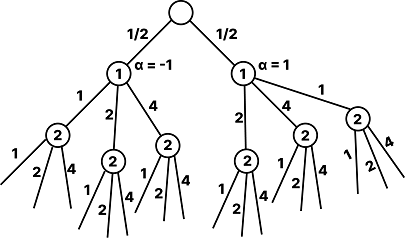
\includegraphics{tree}
\end{center}

راس‌های شامل عدد ۲ اطلاعات یکسان دارند.

\subsection*{ب}

برای یافتن استراتژی بهینه، باید با توجه به تابع سودی هر بازیکن به تحلیل بازی بپردازیم. این یک بازی صفر جمعی است، به این معنی که سود یک بازیکن به اندازه‌ی زیان بازیکن دیگر است. تابع سودی بازیکنان به شکل زیر است:


$$
u_1 = axy , u_2 = - axy
$$

هدف بازیکن اول افزایش
$u_1$ 
و هدف بازیکن دوم کاهش
$u_1$ 
(یا به عبارت دیگر، افزایش
$u_2$
) است.

با توجه به اینکه بازیکنان هر دو می‌توانند از بین اعداد ۱، ۲، و ۴ انتخاب کنند و مقدار a می‌تواند ۱ یا ۱- باشد، انتخاب بهینه برای هر دو بازیکن به شکل زیر است:

بازیکن اول (x) : با توجه به اینکه می‌خواهد
$u_1$ 
را افزایش دهد، باید x را برابر بزرگ‌ترین مقدار ممکن، یعنی ۴، قرار دهد.

بازیکن دوم (y) : با توجه به اینکه می‌خواهد
$u_1$ 
را کاهش دهد (یا
$u_2$ 
را افزایش دهد)، باید y را برابر کوچک‌ترین مقدار ممکن، یعنی ۱، قرار دهد.

بنابراین، استراتژی بهینه برای بازیکن اول
$x=4$
در صورتی که
$\alpha =1$
و در غیر این صورت
۱ را بازی می‌کند،
و برای بازیکن دوم
$y=1$
است.

همچنین لازم به ذکر است که در این تحلیل فرض کردیم که بازیکنان بهینه عمل می‌کنند و از اطلاعات موجود بهترین استفاده را می‌برند. در واقعیت، بازیکنان ممکن است به دلایل مختلف از این استراتژی‌های بهینه منحرف شوند.








	
	\Rule
	
	\item{\textbf{سوال 5.}} \subsection*{آ و پ}

فرم درختی یک روش مدل‌سازی است که برای بازی‌های با توالی زمانی مشخص و تصمیم‌های چندگانه استفاده می‌شود. در این روش، بازی به صورت یک درخت تصمیم‌گیری مدل‌سازی می‌شود. هر گره درخت نماینده یک وضعیت خاص از بازی است و هر یال به یک تصمیم انجام شده و یا عملیاتی که اجرا می‌شود متصل می‌شود. درخت پیمایش می‌شود تا به وضعیت نهایی بازی برسد و نتایج و پاداش‌های متناسب با هر حالت و تصمیم درخت در نظر گرفته می‌شوند. فرم درختی به ما اجازه می‌دهد تا تصمیمات و تأثیرات آن‌ها را به صورت سلسله مراتبی مدل‌سازی کنیم.


از طرفی، فرم نرمال یک روش مدل‌سازی است که برای بازی‌های با توالی زمانی نامعلوم یا همزمان استفاده می‌شود. در این روش، بازی به صورت یک جدول ساده یا نمودار مدل‌سازی می‌شود. در هر سطر از جدول، تمام بازیکنان تصمیمات خود را به صورت همزمان اعمال می‌کنند. هر بازیکن در ستونی از جدول قرار می‌گیرد و نتیجه هر حالت به طور مجزا در نظر گرفته می‌شود. فرم نرمال به ما اجازه می‌دهد تا تعامل‌های همزمان و ناسازگار را در بازی مدل‌سازی کنیم.


ابتدا می‌دانیم که حالت‌های آ و پ یکسان هستند وقتی همزمان تصمیم می‌گیرند A و B ، عملا مانند زمانی‌ست که فرض می‌کنیم انتخاب‌های همدیگر را نمی‌دانند.

استراتژی ز اکیدا مغلوب است و با توجه به بهترین انتخاب‌ها می‌بینیم که سپس ک انتخاب می‌شود در هر دو سمت پس داریم که تعادل زیربازی کامل، (ک و ک) است.

\begin{center}
	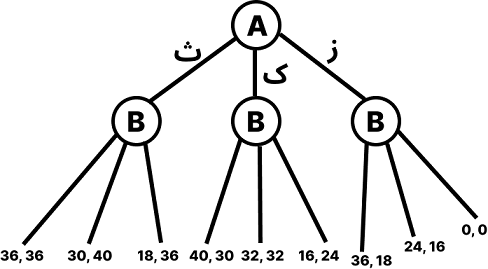
\includegraphics{Tree2}
\end{center}

\begin{center}
	\begin{tabular}{||c c c c||} 
		\hline
		$Z$ & $K$ & $S$ & $$ \\ [0.5ex] 
		\hline\hline
		$18 , 36$ & $30 , 40$ & $36 , 36$ & $S$ \\ 
		\hline
		$16 , 24$ & $32 , 32$ & $40 , 30$ & $K$ \\
		\hline
		$0 , 0$ & $24 , 16$ & $36 , 18$ & $Z$ \\
		\hline
	\end{tabular}
\end{center}


\subsection*{ب}

انتخاب‌های A و ‌B مشخص شده است و تعادل زیربازی کامل، (ز و ث) است.

\begin{center}
	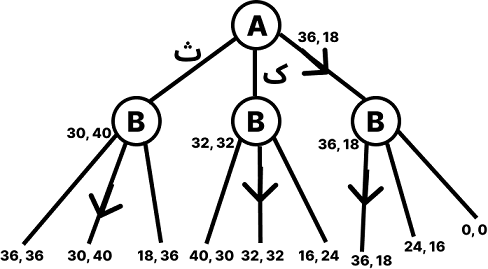
\includegraphics{Tree3}
\end{center}
	
	\Rule
	
	\item{\textbf{سوال 6.}} \subsection*{الف}


X : 4 رأی از گروه A


Y : 2 رأی از گروه C


Z : 3 رأی از گروه B


بنابراین در مرحله اول، گزینه Y با کمترین رأی (2 رأی) حذف می‌شود.


حالا در مرحله دوم، فقط دو گزینه X و Z باقی مانده‌اند. باید دوباره تعداد رأی‌ها را بشماریم با توجه به اینکه گزینه Y حذف شده است.


گروه A هنوز X را به Z ترجیح می‌دهد و 4 رأی به X می‌دهد.


گروه B هنوز Z را به X ترجیح می‌دهد و 3 رأی به Z می‌دهد.


گروه C حالا بر اساس اولویت دوم، Z را به X ترجیح می‌دهد و 2 رأی به Z می‌دهد.


با توجه به اینکه گروه A چهار نفره است و نمی‌تواند در مرحله اول رای گیری با اکثریت رای برنده شود، باید استراتژی خود را تغییر دهد تا در مرحله دوم انتخاب مورد نظر خود را کسب کند.


گروه A می‌داند که اگر در مرحله اول گزینه X را انتخاب کند، با توجه به اینکه گروه B و C با هم 5 رای دارند و در مرحله دوم به گزینه Z رای می‌دهند، گزینه X حذف خواهد شد. پس گروه A برای جلوگیری از حذف گزینه X باید در مرحله اول به گزینه Y رای دهد تا گزینه Z حذف شود.


بنابراین، گروه A باید در مرحله اول به گزینه Y رای دهد. در این صورت، تعداد رای‌ها به شرح زیر خواهد بود:


X : 0 رأی


Y : 4 رأی از گروه A و 2 رأی از گروه C. مجموعاً 6 رأی


Z : 3 رأی از گروه B


در نتیجه، گزینه X با کمترین رأی حذف می‌شود. در مرحله دوم، با حذف گزینه X، گروه A می‌تواند به گزینه مورد علاقه خود یعنی Y رای دهد و این باعث می‌شود گزینه Y با 6 رأی برنده شود. پس گروه A برای اینکه گزینه مورد علاقه‌ی خود را در مرحله دوم انتخاب کند، باید در مرحله اول به گزینه Y رای دهد.


در نهایت، X چهار رأی و Z پنج رأی خواهد داشت. پس گزینه نهایی که انتخاب می‌شود، Z یعنی « عدم تغییر مدیرعامل و افزایش حقوق او » است.
	
	\vspace*{+10ex}\ \hfill\textbf{موفق باشید.}
\end{description}
\end{document}